\begin{figure}[t]
  \centering
  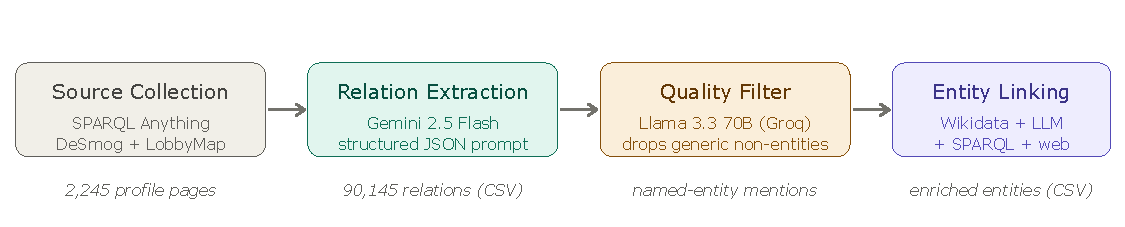
\includegraphics[width=\textwidth]{figures/lack-acquisition-pipeline.pdf}
  \caption{The LACK knowledge acquisition pipeline.
  Each stage is annotated with the model or tool used and the artefact produced.
  The final output feeds into knowledge graph construction (Section~\ref{sec:construction}).}
  \label{fig:acquisition-pipeline}\vspace{-0.3cm}
\end{figure}
\section{Knowledge Acquisition}
\label{sec:extraction}
\paragraph{Requirements and Competency Questions.}
Knowledge requirements were elicited by the authors through informal inductive analysis of ten DeSmog profile pages, manually tagging recurring information types, with emphasis on relations between persons, organisations, and policy actors.
The resulting categories were consolidated into twelve competency questions (CQ1--CQ12) covering four areas (\textit{Transparency and Disclosure}, \textit{Network Structure}, \textit{Temporal Reasoning}, \textit{Identity and Deduplication}), with the resulting ontology subsequently validated for relevance with domain experts (Section~\ref{sec:evaluation}).
The first eleven (CQ1--CQ11) are listed in Table~\ref{tab:coverage} and drove the design of both the ontology (Section~\ref{sec:ontology}) and the extraction pipeline; CQ12, on identity and deduplication, is addressed by the entity linking step described later in this section.
The full text of each question is available on the LACK website\footnote{\url{https://climatesense-project.eu/lack/ontology.html}}.
%
% \paragraph{Sources.}
% LACK was built from the two most comprehensive English-language databases dedicated to climate-lobbying actors\footnote{Pages accessed in December 2025.}; other relevant sources, such as Sceptical Science~\cite{skepticalscience} and SourceWatch, are left to future work.
% \textbf{DeSmog Climate Disinformation Database}~\cite{desmog} is maintained by DeSmog, an international investigative journalism organisation founded in 2006, philanthropically funded, with editorial standards regulated in the UK by IMPRESS, and widely cited by journalists, academics, and policymakers.
% The profile of Cambridge Analytica\footnote{\url{https://www.desmog.com/cambridge-analytica/}}, for example, documents background, fossil fuel connections, funding, key personnel with tenure periods, and a chronological record of notable actions.
% We collected all 943 profile pages listed in the database, typically covering positions on climate science, affiliations, funding sources, and public statements.
% \textbf{LobbyMap}~\cite{lobbymap}, maintained by InfluenceMap (an independent, non-profit think tank founded in 2015), provides analyst-scored assessments of corporate and industry association engagement with climate policy for approximately 1,000 companies and 330 associations, benchmarked against IPCC science.
% The profile of the Business Council of Australia\footnote{\url{https://lobbymap.org/influencer/The-Business-Council-of-Australia}}, for example, provides an overall engagement assessment, a narrative summary of positions across policy areas, a scored evidence matrix by policy query and source, and links to the primary evidence.
% We collected the 964 profile pages from the LobbyMap Scores analysis, plus a further 338 obtained by following links to organisations referenced within them but not themselves in LobbyMap Scores (1,302 pages in total).
% The two sources are complementary: DeSmog focuses on individuals and think tanks involved in active disinformation, while LobbyMap covers corporations and industry associations engaging with policy; well-known actors appear in both.
% The initial set of pages was collected using SPARQL Anything~\cite{daga2021opinionated}, querying the HTML source of the DeSmog Climate Disinformation Database and the JSON feed underlying the LobbyMap Scores leaderboard table.

\paragraph{Sources.}
LACK was built from the two most comprehensive English-language databases dedicated to climate-lobbying actors\footnote{Pages accessed in December 2025.}; other sources, such as Sceptical Science~\cite{skepticalscience} and SourceWatch, are left to future work.
\textbf{DeSmog Climate Disinformation Database}~\cite{desmog}, maintained by DeSmog (an international investigative journalism organisation founded in 2006 and philanthropically funded), profiles individuals and organisations involved in climate denial, typically covering positions on climate science, affiliations, funding sources, and public statements; we collected all 943 profile pages.
\textbf{LobbyMap}~\cite{lobbymap}, maintained by InfluenceMap (an independent non-profit think tank founded in 2015), provides analyst-scored, IPCC-benchmarked assessments of corporate and industry-association engagement with climate policy for approximately 1{,}000 companies and 330 associations; we collected the 964 LobbyMap Scores profiles plus 338 further organisations referenced within them (1,302 pages total).
The two sources are complementary: DeSmog focuses on individuals and think tanks involved in active disinformation, while LobbyMap covers corporations and industry associations engaging with policy; well-known actors appear in both.
The pages were collected using SPARQL Anything~\cite{daga2021opinionated}, querying DeSmog's HTML and the LobbyMap leaderboard JSON feed.

\paragraph{Extraction of relations from web pages.}
Figure~\ref{fig:acquisition-pipeline} summarises the full acquisition pipeline.
The competency questions were translated into a defined set of typed relations between two top-level entity types (Person and Organisation), forming the schema for the extraction pipeline.
Relation extraction was performed by prompting Gemini 2.5 Flash~\cite{gemini25}, chosen for its native URL-context tool (which fetches DeSmog pages directly, avoiding bespoke scraping) and the team's available access.
The prompt specifies the allowed relation types with their definitions, a strict JSON output schema (\texttt{Relation} objects with source, target, type, optional \texttt{xsd:gYear} temporal annotations, a description, and evidence URLs), and a constraint to use only the provided page as evidence.
For DeSmog, page content was fetched directly by the model via Gemini's native URL context tool.
For LobbyMap, HTML pages were fetched separately and passed as input to the model.
The pipeline iterates over all collected profile URLs, invoking the model once per page and storing output as one JSON file per profile, with resumption logic to skip already-processed pages.
After each run, a validation routine identified and deleted malformed or empty outputs; the extraction was then re-run on failed pages, repeating until all pages were successfully processed.
The process, implemented in a Google Colab notebook (deposited~\cite{lack-re}), outputs a CSV file for each data source with a row for each relation, with columns for source, target, their types, relation type, temporal annotations, a natural-language description, and the evidence URL.

\paragraph{Entity Linking.}
The relation extraction step produces entities as surface form strings rather than authoritative identifiers, requiring three further operations: deduplication, entity resolution, and linking to Wikidata~\cite{wikidata}, with Wikipedia as a secondary target or, where no knowledge base entry exists, identification via a dedicated public web page.
The input to this step is a pair of (entity name, evidence link) — the surface form and the source profile page where it appeared — augmented by natural language context sentences aggregated from the previous step.
The same surface form on the same page is treated as a single entity; the same surface form across different pages is not assumed to refer to the same entity.
%A preliminary quality step filters out generic non-entities using Groq-hosted Llama 3.3 70B~\cite{llama33}.
A preliminary quality step filters out generic non-entities using Groq-hosted Llama 3.3 70B~\cite{llama33}, selected for production cost-efficiency at scale.
An LLM classifier distinguishes concrete named entities from purely descriptive or quantitative strings, flagging expressions such as \texttt{"14 lobbyists"}, \texttt{"200 civil society groups"}, or \texttt{"Gas lobby"} for removal, while retaining named events, initiatives, and borderline collectives that carry a proper name.
For the remaining entities, we apply a hybrid linking pipeline combining Wikidata API candidate retrieval, LLM-based disambiguation, and SPARQL-based verification, with a web search fallback for entities absent from Wikidata.
The pipeline was prototyped using Claude Sonnet 4.6~\cite{claudesonnet46}, chosen for stronger reasoning during design, and executed at scale on Llama 3.3 70B~\cite{llama33} (already justified above) for production cost-efficiency; a larger model may have improved recall on long-tail entities, and we leave this comparison to future work.
% For the remaining entities, we apply a hybrid linking pipeline co-designed with Claude~\cite{claude}, combining Wikidata API candidate retrieval, LLM-based disambiguation, and SPARQL-based verification, with a web search fallback for entities absent from Wikidata.
% The pipeline was designed and prototyped using Claude Sonnet 4.6~\cite{claudesonnet46} and executed at scale using Groq-hosted Llama 3.3 70B~\cite{llama33} for cost efficiency.
Candidate Wikidata entries are retrieved via the Wikidata API, with a Wikipedia search API fallback for entities not indexed there, resolving article titles to Wikidata QIDs.
When a Wikipedia page is found, we produce DBpedia resource links.
Because the \texttt{organisation} type in our data spans a wide range of entity classes — companies, think tanks, PACs, government agencies, events, journals, and coalitions — type-based filtering in Wikidata is unreliable; entity subtype is instead inferred by the LLM from context.
Candidates are passed to the LLM, which selects the best matching QID or returns null, also detecting when a candidate represents a broader parent entity rather than the specific entity itself.
Selected QIDs are verified via SPARQL, retrieving canonical label, Wikipedia sitelink, and parent organisation (via \texttt{P749}/\texttt{P361}).
For entities with no Wikidata match, a web fallback first evaluates the evidence link as a potential primary identifier, then issues an LLM-generated search query via the Google Custom Search API~\cite{googlecse}, with a primary-subject check confirming whether each result page is dedicated to the entity.
The output is an enriched CSV of entities, containing Wikidata URIs, Wikipedia URLs, parent entity links, web page fallbacks, and confidence scores. All code and data are published~\cite{lack-el}.

\paragraph{Evaluation of the extraction output.}
We now evaluate the extracted data: source coverage, the accuracy of extracted relations and entity links, and known limitations.

Our collection covers the DeSmog Climate Disinformation Database and the LobbyMap Scores leaderboard in their entirety as of the time of collection, providing complete coverage with respect to these two curated entry points.
With respect to LobbyMap, the Scores leaderboard covers approximately 1,000 companies and 330 industry associations, but InfluenceMap hosts a broader set of content — including sector-level reports, country profiles, and policy engagement assessments — that was not included in the current collection.
Extending coverage to these additional sources remains a direction for future work.

Relation extraction was evaluated on a sample of 300 relations drawn from 8 randomly selected DeSmog profile pages.
Three annotators (the authors) worked in pairs, each pair covering approximately 100 relations, with disagreements resolved by discussion.
Each relation was assessed on three dimensions: truthfulness (is the relation supported by the source page?), validity (is the relation type and its domain and range correctly applied according to the schema?), and temporal correctness (are the temporal annotations accurate?)\footnote{Full annotation guidelines: \url{https://bit.ly/lack_42bhqzl}.}.
Truthfulness accuracy is 0.93 (0.99 with partial credit), validity 0.907 (0.95 with partial), and temporal correctness 0.797 (0.91 with partial), where partial credit captures approximately correct extractions.
The main source of partly correct answers relates to the conflation of specific sub-roles with the coarser schema relations: the model frequently uses \texttt{is president of} or \texttt{is director of} where the source text indicates a more specific role such as vice-president, deputy director, or departmental director.
A recurrent validity issue is the misapplication of organisation-level relations to person-organisation pairs: for example, \texttt{has partner} was used when a person holds a partner title at a law or consulting firm, whereas the relation was intended to connect two organisations in a formal partnership.
Temporal correctness is the least accurate dimension, with errors arising from missing dates, incorrect inference of date ranges, and ambiguity in encoding point-in-time vs.\ interval information, but still reaching ~0.80\% of accuracy.

Entity linking was evaluated on 225 entities from the same pages as the previous evaluation, against a curated gold standard\footnote{Gold standard preparation: \url{https://bit.ly/lack_3QQPRsD}} produced by four annotators (the authors), each covering approximately 56 entities, with a subset supervised by a second annotator and disagreements resolved by discussion.
Each entity was assessed on five dimensions: entity subtype correctness, Wikidata URI, Wikipedia URL, parent entity, web page (where applicable); see-also links were assessed separately.
Accuracy is high across most dimensions, with see-also at 0.96, parent entity at 0.94, Wikidata URI and Wikipedia URL at 0.88, entity subtype at 0.86, and web page at 0.84, indicating that the pipeline reliably identifies and links entities across all primary output fields.
For the two fields whose gold reference can be precisely defined---Wikidata URI and Wikipedia URL---precision and recall are also balanced (0.93/0.85 and 0.88/0.88 respectively), confirming that the pipeline neither over- nor under-produces links for these dimensions.
The weakest dimension in terms of precision is web page (0.49 precision, 0.59 recall), reflecting the difficulty of identifying a single canonical web presence.
Parent entity, despite high overall accuracy, exhibits the most informative error pattern (precision 0.79, recall 0.73): the dominant failure mode is over-eager parent assignment for foundations, transition teams, and political campaigns where no real parent organisation exists in Wikidata, alongside a smaller number of cases in which a meaningful parent was missed entirely.
Of the 219 entities with see-also content in the gold standard, only 19 included at least one novel URL beyond the evidence link, contributing 44 additional reference pages in total ($\approx 8.4\%$).

Of the 27,945 entities in the KG, 10,189 (36.5\%) are linked to Wikidata or DBpedia, while 17,756 (63.5\%) remain without an external identifier --- a proportion that is consistent across both sources: 64.4\% of DeSmog-only entities and 65.7\% of LobbyMap-only entities are NIL.
This high NIL rate is not a pipeline failure but a domain characteristic: the climate lobbying ecosystem is densely populated with minor think tank staff, obscure industry consultants, short-lived coalitions, and regional trade bodies that are simply not represented in general-purpose knowledge bases such as Wikidata.
By contrast, entities appearing in both sources --- those prominent enough to be independently documented by DeSmog and LobbyMap --- are linked at a rate of 95.7\% (488 out of 510), confirming that the pipeline reliably identifies well-known actors.
NIL entities will be resolvable within the KG via their LACK URI and retain their label and source provenance; web page and parent entity fields, included as \textit{see also} statements, captured during entity linking but not yet promoted to \texttt{owl:sameAs} assertions, offer a path to further grounding and are left to future work.
A residual data quality issue --- 29 entities with inconsistent type assignments across pages --- will be resolved in a future release.

